\pickl{18.04.2024}
\subsubsection{Bemerkung}
Wie findet man nun das richtige Wahrscheinlichkeitsma\ss{}, d.h. jenes, welches zu meinem Experiment passt?
\num{
\item Ausprobieren (siehe unten, ``Statistik'').
\item Analyse der physikalischen Eigenschaften. Praktikabel, falls Symmetrie in den relevanten physikalischen Eigenschaften herrscht:
}
\subsubsection{Laplace-Annahme (Indifferenzprinzip)}
Falls es keinen Grund zur Annahme gibt, dass die verschiedenen Ausg\"ange des Experiments im Wesentlichen zu unterscheiden sind, nehmen wir an, dass die Wahrscheinlichkeiten aller Elementarerignisse gleich sind.
\subsubsection{Folgerung}
Sei $\Omega$ ein Ergebnisraum. Unter der Laplace-Annahme gilt:
\meq{
\PP(A)=\frac{|A|}{|\Omega|}
}
\subsubsection{Beweis}
\meq{1\textabove{\tbf{K}}{=}\PP(\Omega)=\PP(\bigcup_{\omega\in\Omega}\{\omega\})\textabove{\tbf{K}}{=}\sum_{\omega\in\Omega}\PP(\{\omega\})\textabove{\tbf{L}}{=}|\Omega|\cdot\PP(\{\omega\})}
$\RA\forall\omega\in\Omega$ gilt:
\meq{\PP(\{w\})=\frac{1}{|\Omega|}.}
Au\ss{}erdem:
\meq{\PP(A)=\PP(\bigcup_{\omega\in A}\{\omega\})\textabove{\tbf{K}}{=}\sum_{\omega\in A}\PP(\{\omega\})=|A|\cdot\frac{1}{|\Omega|}.}
\subsubsection{Beispiel}
\num{
\item Werfen eines ungezinkten W\"urfels:
\meq{\PP(\{2,4,6\})=\frac{3}{6}=\frac{1}{2}.}
\item Gesamte Augenzahl bei zweimaligen Werfen des W\"urfels
\meq{\Omega=\{2,\ldots,12\},}
Laplace-Annahme gilt nicht. Die Elemente sind wesentlich verschieden, z.B. $2$ hat nur Option $(1,1)$, $7$ hat die Optionen $\{(1,6),\ldots\}$.
\item Ziegenproblem: Wir befinden uns in einer Gameshow, d\"urfen zwischen drei Toren w\"ahlen. Hinter einemal Tor ist ein Gewinn, hinter zweien eine Niete. Der Moderator \"offnet eines der nicht-gew\"ahlten Tore. Hinter diesen ist eine Niete. Er bietet daraufhin an, das Tor zu wechseln. Ist der Wechsel sinnvoll?
\bul{
\item Problem 1: Spielregeln m\"ussen erg\"anzt werden. Wie handelt der Moderator? Wir gehen davon aus, dass er oder sie in jedem Fall ein nicht-gew\"ahltes Tor mit Niete \"offnet.
\item Problem 2: Man ist geneigt, von einer Laplace-Situation auszugehen. Dies ist falsch, da die Tore durch die Wahl und die Reaktion des Moderators zu unterscheiden sind.
}
}
\begin{center}
\begin{minipage}{0.45\textwidth}
\centering
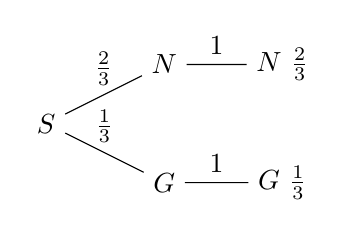
\begin{tikzpicture}[grow=right]
    \node {$S$}
        child
        {
            node {$G$}
            child
            {
                node {$G\ \frac{1}{3}$}
                edge from parent node[above] {$1$}
            }
            edge from parent node[above] {$\frac{1}{3}$}
        }
        child
        {
            node {$N$}
            child
            {
                node {$N\ \frac{2}{3}$}
                edge from parent node[above] {$1$}
            }
            edge from parent node[above] {$\frac{2}{3}$}
        };
\end{tikzpicture}\\
Ohne Wechseln
\end{minipage}
\begin{minipage}{0.45\textwidth}
\centering
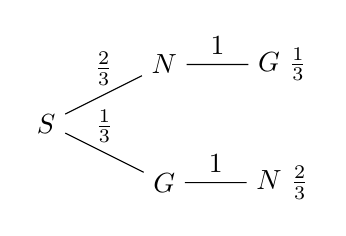
\begin{tikzpicture}[grow=right]
    \node {$S$}
        child
        {
            node {$G$}
            child
            {
                node {$N\ \frac{2}{3}$}
                edge from parent node[above] {$1$}
            }
            edge from parent node[above] {$\frac{1}{3}$}
        }
        child
        {
            node {$N$}
            child
            {
                node {$G\ \frac{1}{3}$}
                edge from parent node[above] {$1$}
            }
            edge from parent node[above] {$\frac{2}{3}$}
        };
\end{tikzpicture}\\
Mit Wechseln
\end{minipage}
\end{center}
mit Start ($S$), Gewinn ($G$) und Niete ($N$).
\subsection{Kombinatorik}
Wie bestimmt man in einer Laplace-Situation $|A|$ und $|\Omega|$?
\subsubsection{Beispiele}
\abc{
\item Sei $\Omega=A\times B$, so ist $|\Omega|=|A|\cdot|B|$ M\"unzwurf, dann W\"urfel:
\meq{A=\{\text{K},\text{Z}\},\ B=\{1,\ldots,6\}.}
\item Urne mit $N$ durchnummerierten Kugeln. Wir ziehen davon nacheinander ohne Zur\"ucklegen $k$ Kugeln (Reihenfolge wird ber\"ucksichtigt):
\meq{|\Omega|=N(N-1)\ldots(N-k+1)=\frac{N!}{(N-k)!}.}
\item Zahlenlotto ``6 aus 49'', wie b) ohne R\"ucksicht auf Reihenfolge:
\meq{|\Omega|=\frac{N!}{(N-k)!}\cdot\frac{1}{k!}.}
\item Anzahl der Anagramme von \ttt{MISSISSIPPI}.
\meq{|\Omega|=\frac{11!}{\ubr{4!}{\ttt{I}}\ubr{4!}{\ttt{S}}\ubr{2!}{\ttt{P}}}.}
}
\newpage
\section{Allgemeine Wahrscheinlichkeitsr\"aume}
\setcounter{subsection}{-1}
\subsection{Anpassung des 3. Axioms von Kolmogorov}
Wir werden das 3. Axiom von Kolmogorov anpassen:
\meq{\PP(\bigcup_{j=1}^\infty A_j)=\sum_{j=1}^\infty\PP(A_j),\ \text{falls}\ A_j\cap A_k=\emptyset,\ \forall j\neq k.}
Schwieriger ist die anpassung des Definitionsbereiches von $\PP$. Warum ist das n\"otig? Betrachte das Beispiel ``Gl\"ucksrad''. 
